\documentclass[10pt,letterpaper,notitlepage]{article}
\usepackage{graphicx}
\usepackage[margin=1in]{geometry}
\usepackage{hyperref}
\hypersetup{colorlinks=true}
\usepackage{amssymb,amsfonts,amsmath,upgreek}
\renewcommand{\familydefault}{\sfdefault}
\usepackage{listings}
\usepackage{courier}
 \lstset{
         basicstyle=\footnotesize\ttfamily, % Standardschrift
         numberstyle=\tiny,          % Stil der Zeilennummern
         numbersep=5pt,              % Abstand der Nummern zum Text
         tabsize=2,                  % Groesse von Tabs
         extendedchars=true,         %
         breaklines=true,            % Zeilen werden Umgebrochen
         keywordstyle=\color{red},
    		frame=b,         
         stringstyle=\color{white}\ttfamily, % Farbe der String
         showspaces=false,           % Leerzeichen anzeigen ?
         showtabs=false,             % Tabs anzeigen ?
         xleftmargin=17pt,
         framexleftmargin=17pt,
         framexrightmargin=5pt,
         framexbottommargin=4pt,
         showstringspaces=false      % Leerzeichen in Strings anzeigen ?        
 }
\setlength{\parskip}{\baselineskip}%
\usepackage{caption}
\usepackage{bm}
\DeclareCaptionFont{white}{\color{white}}
\DeclareCaptionFormat{listing}{\colorbox[cmyk]{0.43, 0.35, 0.35,0.01}{\parbox{\textwidth}{\hspace{15pt}#1#2#3}}}
\captionsetup[lstlisting]{labelformat=empty,format=listing,labelfont=white,textfont=white, singlelinecheck=false, margin=0pt, font={bf,footnotesize}}
%opening
\parindent=0mm


\begin{document}
\title{Computing the Local Stress Tensor in MD \\Simulations of Biomolecules}
\author{Juan M.~Vanegas and Alejandro Torres-S\'anchez
\\juan.m.vanegas@gmail.com
\\torres.sanchez.a@gmail.com
\\Universitat Polit\`ecnica de Catalunya-BarcelonaTech, \\Barcelona, Spain.}
\maketitle

\section{Introduction}
This is a manual for our Custom GROMACS version to compute the local stress tensor in 3D over a simulation, GROMACS-LS. This program computes the local stress based on the Hardy stress definition (see Ch.8 in Tadmor \& Miller (2011) {\bf Modeling Materials: Continuum, Atomistic and Multiscale Techniques}). It can also be used to compute the atomic virial stress (A. P. Thompson et al., J. Chem. Phys. 131, 154107 (2009)). We have patched the GROMACS source code (v4.5.5) at various locations in the routines that calculate particles forces and velocities. Our patches rely heavily on the code structure and functions implemented in a previous local pressure code (obtained from \url{http://repo.or.cz/w/gromacs.git/shortlog/refs/heads/release-4-5-localpressure} and \url{ftp://ftp.gromacs.org/pub/tmp/gromacs-4.0.2_localpressure.tar.gz}). This previous code implements the methodology outlined in

{\bf 3D Pressure Field in Lipid Membranes and Membrane-Protein Complexes} by S. Ollila et al. Phys. Rev. Lett. 102, 078101 (2009). 

In the current custom GROMACS version we implement the methodology outlined in

{\bf Importance of Force Decomposition for Local Stress Calculations in Biomembrane Molecular Simulations} by J. M. Vanegas, A. Torres-Sanchez, and M. Arroyo. J. Chem. Theor. Comput.  10, 691 (2014). 

and in

{\bf Is the stress tensor computed from molecular simulations in mechanical equilibrium?} by  A. Torres-S\'anchez, J. M. Vanegas, and M. Arroyo. Submitted to PRL (2015).

The main differences of our implementation compared the previous one include:
\begin{itemize}
    \item Decomposition of multi-body potential forces using:
    \begin{enumerate}
	\item Covariant central force decomposition (cCFD) (Torres-S\'anchez A. Vanegas, J. and Arroyo, M. (in preparation)).
    \item Non-covariant central force decomposition (nCFD) (N. C. Admal and E. B. Tadmor; J. Elast. 100, 63-143, 2010).
    \item Goetz-Lipowsky decomposition (GLD) (R. Goetz and R. J. Lipowsky; J. Chem. Phys. 108, 7397-7409, 1998.). 
    \item Decomposition on geometric centers (Heinz, A.  Paul W. and Binder K. Phys. Rev. E. 72 066704 (2005)).
    \end{enumerate}
\item Ability to output the total or individual contributions to the local stress such as those from vdw, electrostatics, angles, and others.
\item Finite discretization over a rectangular grid using tri-linear weight functions, which result in smoother stress fields and also make the discretization exact regardless of the grid size.
\item Consistent treatment of forces arising from bond constraints (LINCS, SETTLE and SHAKE algorithms), which produces constant profiles for the normal component (perpendicular to the membrane plane) of the stress. This is necessary from an equilibrium stand-point and was an unresolved problem for stress profiles obtained from atomistic membrane simulations.
\item Virial stress per atom. In the last version we have included the
calculation of the virial stress per atom as defined in
A. P. Thompson et al., J. Chem. Phys. 131, 154107 (2009). The computation of the virial stress per atom is much faster than the 
computation of the IKN stress in a grid.
\end{itemize}
If you publish results using this code, we kindly ask you to cite the papers by Ollila et al., Vanegas et al., and Torres-S\'anchez et al., which we recommend you to read before continuing with the rest of the manual. In these papers we show the main differences between the different definitions of the stress. We show that the virial stress per atom and the stress from the decomposition on geometric centers do not satisfy balance of linear momentum, while the stress from cCFD, nCFD and GLD do. We also show that the GLD and the stress from the decomposition on geometric centers lead to non-symmetric stresses, which therefore do not satisfy balance of angular momentum. The two flavors of the CFD do satisfyboth balance of linear and angular momentum by construction. However, for potentials beyond 4-body, such as the CMAP interaction, the nCFD leads to unphysical stresses. We therefore suggest that the cCFD definition is preferred in any case.

The types of interaction potentials that are included in stress calculations and have been tested are the following:

\begin{itemize}
\item Bonds
\item Angles
\item Dihedrals (proper, improper, and Ryckaert-Bellemans)
\item Constraints (SETTLE and LINCS, SHAKE is included but has not been tested)
\item Van der Waals
\item Coulomb (plain cut-off and reaction-field) 
\item CMAP
\end{itemize}

As such, if you use this code to analyze a system that may use other types of potentials, we cannot guarantee that it will be correct. Please thoroughly check the output of the program and compare to known quantities such as the total pressure. For such comparisons you should first reanalyze the trajectory (i.e. \texttt{mdrun\_d -rerun}) using a double precision version and recompute the pressure with \texttt{g\_energy\_d}.

\section{Installation}

This code is based on Gromacs version 4.5.5. While the vanilla 4.5.5 version can be compiled using both the \texttt{autoconf} tools and \texttt{cmake}, this custom version can only be compiled with \texttt{cmake}. You will need to install a recent version of the FFTW library (in double precision) and CMake. If you install these programs with a linux distribution such as Ubuntu or Fedora, you will also need to install the development (header) packages. After extracting the \texttt{.tar.gz} package, create a build directory and launch \texttt{ccmake} from within this folder:
\begin{lstlisting}[caption=Basic compilation instructions with CMake]
$ tar -zxvf gromacs-4.5.5-LS.tar.gz
$ cd gromacs-4.5.5-LS
$ mkdir build
$ cd build
$ ccmake ../
\end{lstlisting}
If you have installed the FFTW library in a non-standard location (i.e. other than /usr/lib or /usr/local/lib), then before running \texttt{ccmake} you should export the variable \texttt{FFTW3\_ROOT\_DIR}, e.g. 

\bigskip
\texttt{export FFTW3\_ROOT\_DIR=/share/apps/modules/fftw/3.3}.
\bigskip

The new version of the code also requires an external LAPACK library, whose path must be given to cmake in case of not being standard (e.g.~/usr/lib)

\bigskip
\texttt{export CMAKE\_PREFIX\_PATH=/path/to/lapack/lib}
\bigskip

Once the \texttt{ccmake} dialog comes up, press c to begin the initial configuration, and then modify the \texttt{CMAKE\_INSTALL\_PREFIX} variable to set the target installation directory. Do not modify other variables unless you know what you are doing. By default, the code is compiled in double precision (this is absolutely necessary), it cannot be compiled with MPI or GPU support, and all programs have the suffix \texttt{\_LS}. Press c again and then g to generate the necessary Makefiles. After \texttt{ccmake} quits you can follow the standard linux installation commands of \texttt{make} and \texttt{make install}

In addition to the Gromacs code, we have also include two utilities in the \texttt{tensortools} folder of the source code. These are two python tools: \texttt{LStensor.py} and \texttt{tensortools.py}. The first defines a \texttt{LStensor} object that you can use for your own python scripts. The second uses the first to create a tool for simple use that performs different useful post-processings (averagind, smoothing, storing in different formats, etc) to the stress fields obtained from the GROMACS code. We discuss these tools in more detail in Section \ref{postprocess}. Both tools are installed in the GROMACS bin folder during the compilation of the code.

\section{Using the Code}

\subsection{Analyzing an MD Trajectory}

For calculating the stress tensor in a MD simulation, we need a trajectory file (\texttt{.trr}) that contains both positions and velocities at the same points in time. In this section we show the steps you need to follow to calculate the stress tensor and illustrate it in the particular case of a POPE membrane. 

As individual components of the system may drift over time, e.g. a membrane may drift in the simulation box, it is a good idea to first center a given group of atoms (in this case, the POPE bilayer) in the center of the simulation box. To do so, we use the tool \texttt{trjconv\_LS} with the original trajectory, \texttt{traj.trr}:
\begin{lstlisting}[caption=Center the molecule into the simulation box before analyzing the stress]
$ trjconv_LS -f traj.trr -o traj_centered.trr -n index -center -s topol.tpr

(...)

Select group for centering
Group     0 (         System) has 11600 elements
Group     1 (           POPE) has  2600 elements
Group     2 (          Water) has  9000 elements
Select a group: 1
\end{lstlisting}
Note that this \texttt{trjconv\_LS} is a modified version of the vanilla one that places the center of mass, and not the geometrical center as it is done by the original, of the selected index group at the center of the simulation box. You must always pass a \texttt{.tpr} file as part of the input, or the program will return a segmentation fault without an error message. This new \texttt{traj\_centered.trr} is the trajectory we will use to analyze the stress.

The 3D stress tensor is obtained by ``rerunning'' the trajectory with the \texttt{mdrun\_LS}. Since the \texttt{-rerun} option of \texttt{mdrun\_LS} outputs new \texttt{.log}, \texttt{.edr}, and \texttt{.trr} files, we suggest you first create a new folder and analyze the trajectory within it:
\begin{lstlisting}[caption=Computing the stress with \texttt{mdrun\_LS}]
$ mkdir stress
$ cd stress
$ mdrun_LS -s ../topol.tpr -rerun ../traj_centered.trr
\end{lstlisting}
To save space you can recreate the \texttt{.tpr} file by setting all the output \texttt{nst*} variables to 0 in the \texttt{.mdp} file:

\texttt{
\footnotesize{
\\nstxout         = 0\\
nstvout         = 0\\
nstlog          = 0\\
nstenergy       = 0\\
nstxtcout       = 0\\
}}

If your simulation was performed with PME or another long-range electrostatic method, you will need to create a new \texttt{.tpr} file with the \texttt{coulombtype} set to \texttt{Cut-off} or \texttt{Reaction-field} and a cutoff radius of at least 2.0-2.2 nm (see the Ref. 2 for more details). Note that this does not change your original trajectory but the way forces are calculated when analyzing each frame.

As with other Gromacs tools, \texttt{mdrun\_LS} displays a help text running \texttt{mdrun\_LS -h}. \texttt{mdrun\_LS} has several special options for analyzing the stress:
\begin{lstlisting}[caption=\texttt{mdrun\_LS} special options]
Option     Filename  Type         Description
------------------------------------------------------------
-ols localstress.dat  Output       Generic data file

Option       Type   Value   Description
------------------------------------------------------
-localsgrid  real   0.1     Spacing for local pressure grid (default = 0.1 nm)
-lsgridx     int    0       Set the local pressure grid size in the x
                            direction (default use box[XX][XX]/localsgrid)
-lsgridy     int    0       Set the local pressure grid size in the y
                            direction (default use box[YY][YY]/localsgrid)
-lsgridz     int    0       Set the local pressure grid size in the z
                            direction (default use box[ZZ][ZZ]/localsgrid)
-lscont      string all     Select which contribution to write to output
                            (default = all): all, vdw, coul, angles, bonds,
                            dihp, dihi, dihrb, lincs, settle, shake, vel
-lsfd        string ccfd    Select the type of force decomposition to be
                            used: ccfd (covariant central force
                            decomposition, default), ncfd (non-covariant
                            central force decomposition), gld (Goetz-Lipowsky
                            decomposition), or gmc (decomposition on
                            geometric centers)
-lssa        string spat    Select the type of stress to calculate: spat
                            (spatial stress from IKN theory, default), atom
                            (stress per atom)

\end{lstlisting}
With the flag \texttt{-ols} one selects the output file where the stress tensor is stored. The size of the discretization grid is given by several parameters. If your system was simulated at constant pressure, the program takes the size of the box (box[XX], box[YY], box[ZZ]) from the \texttt{.tpr} along with the desired grid spacing (with \texttt{-localsgrid}), and calculates the integer size of the grid and the real grid spacing, e.g. if the box size in the x direction is 5.37 nm and the given grid spacing is 0.1 nm, then the grid size in x is 53 and the real grid spacing becomes 0.1013 nm. The grid size in each dimension can also be overridden with the \texttt{-lsgridx}, \texttt{-lsgridy}, or \texttt{-lsgridz}. So if you are interested in calculating a stress profile along a given dimension, e.g. z, then you can use these different flags together:
\begin{lstlisting}[caption=Setting the grid size]
$ mdrun_LS -s ../topol.tpr -rerun ../traj_centered.trr -localsgrid 0.1 -lsgridx 1 -lsgridy 1
\end{lstlisting}
%check to use simulations with non-rectangular boxes - use trjconv to change
At the moment, only systems simulated with rectangular boxes can be analyzed. \texttt{mdrun\_LS} can also return the total or individual contributions to the stress with the \texttt{-lscont} flag. At the moment the available contributions are van der Waals, Coulomb, angles, bonds, proper dihedrals, improper dihedrals, Ryckaert-Bellemans dihedrals, constraints (LINCS, SHAKE, or SETTLE), and kinetic. 

Finally, the \texttt{-lsfd} flag allows to select one of two different decompositions for the forces between particles that enter into the potential part of the stress. We advice you to use the ccfd option (set by default in the program) that always provides a symmetric stress, thereby satisfying the balance of angular momentum from a continuum viewpoint, and physically meaningful regardless of the number of particles involved in each additive potential of the force field. The ncfd is equivalent to the ccfd except for 5-body potentials. On the other hand, the gld option allows you to compute the stress from the decomposition by Goetz and Lipowsky (J. Chem. Phys. (1998) 17, 7397-7409), which has been widely used in biomembrane simulations. Please, take a close look to references 2 and 3 for a more detailed discussion about the differences between both decompositions.


The outputted \texttt{.dat0} file is a simple binary file in double precision with the following format:
\begin{lstlisting}[caption=Format of the \texttt{.dat0} binary file]
precission   = sizeof(int)*1
box          = sizeof(double)*9
gridx        = sizeof(int)*1
gridy        = sizeof(int)*1
gridz        = sizeof(int)*1
stresstensor = sizeof(double)*9*gridx*gridy*gridz
\end{lstlisting}

\subsection{Python scripts to post-process the stress fields \label{postprocess}}

The command \texttt{mdrun\_LS} produces \texttt{.dat0} files that need to be loaded properly for analysis. To make the life easier, we have included two tools that can load, transform and save in useful formats the raw \texttt{.dat0} files. These files are directly installed to the binary folder of the GROMACS\_LS distribution. 
\subsubsection{LStensor}
The LStensor.py file encapsulates the LStensor object, which can be used to post-process the data from the GROMACS\_LS program. This object can load IKN stresses as well as stresses per atom and convert these to a grid. It can also be used to compute the basic invariants of the stress as well as its divergence. It also provides a number of functions to load PDB files and to store files in NetCDF format, txt format and PDB format.

\subsubsection{tensortools}
Tensor tools can be used for a rapid post-processing of the data. It loads a LStensor object with which it operates. The main options are:
\begin{lstlisting}[caption=Options for tensortools (tensortools -h)]
-h, --help            show this help message and exit
-f [input.bin] [[input.bin] ...]
                      Single or multiple binary input files (must all have
                      the same grid size)
-v []                 verbose
--irep [spat]         Input data representation, values: spat (spatial
                      stress/density distributed on a grid, default), atom
                      (stress per atom)
--pdb [[structure.pdb]]
                      PDB file with atom coordinates (FOR STRESS PER ATOM
                      ONLY)
--itype [stress]      Type of data such as density, stress tensor, or vector
                      field: dens, stress (default), or vec
--mif [avg]           How to process multiple input files, values: avg
                      (default) or sum
--sym []              FOR STRESS ONLY. Separates the resultant stress in its
                      symmetric and antisymmetric parts, and creates two
                      outputs with the subscripts _sym and _asym
                      respectively
--prof z              Output a profile along a given dimension, values: x,
                      y, or z (default)
--integ z             integrate out the stress profile along a given
                      dimension, values: x, y, or z (default)
--gf 1.0              Process input through a gaussian filter of a given
                      width (in units of the grid spacing, default=1.0)
--gridsp 0.1 0.1 0.1  (For atom to grid conversion) Grid spacing for atom 2
                      grid conversion (default 0.1, 0.1, 0.1 nm)
-o output.bin         Output file
--orep [spat]         Output data representation, values: spat (spatial
                      stress/density distributed on a grid, default), atom
                      (stress per atom)
--oformat [bin]       Output format, values: bin (i.e. binary .dat0,
                      default), nc (NETCDF), txt or pdb (stress per atom only - 
                      creates a separate file for each element in the tensor)
  
\end{lstlisting}
Some examples of usage:
\begin{lstlisting}[caption={Read the IKN stress from *.dat0 files, integrate out the z direction, smooth the data with a Gaussian filter of 25 (units of the grid size), and write the result in the file stress\_gf25.nc}]
tensortools -f *.dat0 --inte z --oformat nc --gf 25 -o stress_gf25.nc -v
\end{lstlisting}

\begin{lstlisting}[caption={Read the stress per atom from *.dat0 files, load the PDB structure from struct.pdb, translate the data to a grid with spacing 0.01, 0.01, 10, apply a Gaussian filter of 25 and store the result in stress\_atom\_gf25.nc}]
tensortools -f *.dat0 --irep atom --pdb struct.pdb  --orep spat --oformat nc -o stress_atom_gf25.nc --gridsp 0.01 0.01 10 --gf 25 -v
\end{lstlisting}


\subsection{Visualizing the Stress Tensor}
As most programs cannot directly read the binary files that \texttt{mdrun\_LS} outputs, we also provide several small utilities to convert the data into other formats more adept for visualization. These programs are available in the \texttt{tensortools} folder of the downloaded source (see the Installation section). The \texttt{bin2xvg} is a specific tool to obtain stress profiles from simulations of membranes in which the direction normal to the membrane plane is the z axis. This program takes as input a \texttt{.dat0} file and outputs a plain text file (\texttt{.xvg}) with the 9 elements of the pressure tensor, $P_{ij}(z)=-\sigma_{ij}(z)$ (for convenience, see below), along the z axis:
\begin{lstlisting}[caption=\texttt{bin2xvg} usage]
$ bin2xvg input_1.dat0 ... input_n.dat0 output.xvg
$ head -n 2 output.xvg
# Pij(z) = -sigma_ij(z)
# Zcoord in nm 	 Pxx(z) Pxy(z) Pxz(z) Pyx(z) Pyy(z) Pyz(z) Pzx(z) Pzy(z) Pzz(z) in bar
0.0000	22.23	-1.08	-0.67	-1.08	12.34	-4.35	-0.67	-4.35	23.09
\end{lstlisting}
This program can take many \texttt{.dat0} input files at the same time and average them together. However, please use this with caution as the program will always write the output data to the last file given, even if that file already exists. So, if you forget to specify the name of the output file, it will overwrite the last input file.

Stress profiles for a 200 lipid POPE membrane simulated with both the Martini force field (FF) and the atomistic Gromos 43A1-S3 FF (see Ref. 1) are shown in Figure 1. Please note that the continuum mechanics convention is different from that commonly used to display lateral pressure profiles. The lateral component is defined as $P_L=-(\sigma_{xx}+\sigma_{yy})/2$ and the normal component as $P_N=-\sigma_{zz}$, where $\bm{\sigma}$ is the stress tensor.

\begin{figure}[b]
\centering
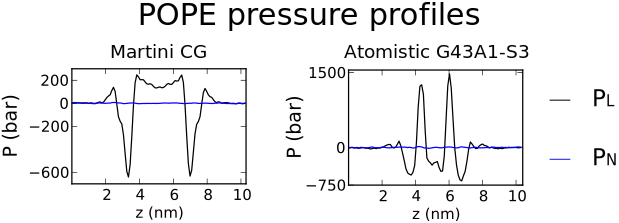
\includegraphics[width=5.5in]{figs/tot.pdf}
\caption{}
\end{figure}

A second program, \texttt{bin2ncdf}, can be used to convert the 3D stress tensor (not the pressure tensor) into the NETCDF file format that can be loaded into many visualization programs such as UCSF Chimera or ParaView:
\begin{lstlisting}[caption=\texttt{bin2ncdf} usage]
$ bin2ncdf input_1.dat0 ... input_n.dat0 output.nc
\end{lstlisting}
The $\sigma_{xx}$ component of the stress in 3D is shown in Figure 2 for the atomistic POPE system. Other NETCDF utilities such as \texttt{ncdump} can also be used to further process the \texttt{.nc} file. An example of the partial contribution of the stress (\texttt{-lscont}) is shown in Figure 3 for both coarse-grained and atomistic systems. The convergence of the computed stress tensor depends on the system analyzed. For biomembranes, we recommend to analyze a trajectory of 50-100 ns, with the positions and velocities saved every 5-10 ps. Figure 4 shows the convergence of stress profiles for an atomistic DPPC simulation of 100 ns with frames saved every 5 ps.

\begin{figure}
\centering
\includegraphics[width=4in]{figs/3D_stress_black_bw.pdf}
\caption{}
\end{figure}

\begin{figure}
\centering
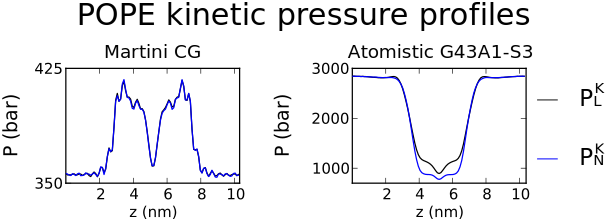
\includegraphics[width=4in]{figs/kin.pdf}
\caption{}
\end{figure}



\begin{figure}[h]
\centering
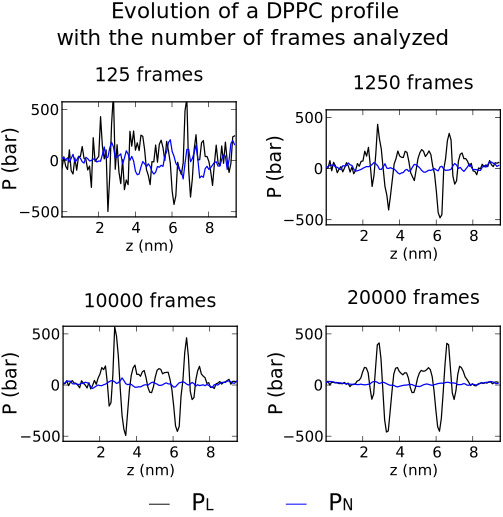
\includegraphics[width=4in]{figs/evol.pdf}
\caption{}
\end{figure}

\begin{figure}[h]
\centering
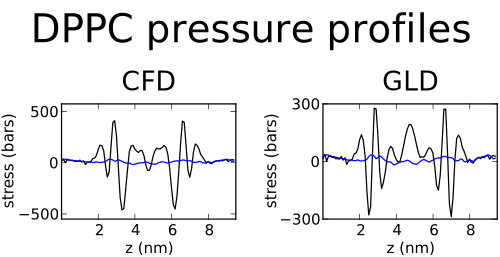
\includegraphics[width=4in]{figs/CFD_GL.pdf}
\caption{}
\end{figure}

\section{Some technical comments about cCFD and nCFD}

In the new version of the code, computing any flavor of the central force decomposition (cCFD and nCFD) for a given potential $V_I$ is done by solving the overdetermined system of equations
\begin{equation}
\label{system}
\bm{F}_I^\alpha = \sum_{\beta\in\mathcal{I}_I,\beta\neq\alpha}  \bm{f}^{\alpha\beta}= \sum_{\beta\in\mathcal{I}_I,\beta\neq\alpha}  \varphi^{\alpha\beta}\frac{\bm{r}^{\alpha\beta}}{|\bm{r}^{\alpha\beta}|}, \forall \alpha \in \mathcal{I}_I
\end{equation}
where $\mathcal{I}_I$ is the set of particles interacting through the potential $V_I$, $\bm{f}^{\alpha\beta}$ are the terms of the force decomposition and $\varphi{\alpha\beta}$ are their respective magnitudes. If $n_I$, the number of particles involved in the potential, is equal or smaller than 4, this overdetermined system has a single solution and thus cCFD and nCFD coincide. For potentials beyond 4-body, such as the CMAP interaction, this systems becomes underdetermined with an infinite number of possible solutions. We have recently proposed a preferred CFD based on covariance arguments (Torres-S\'anchez et al., in preparation), which we call cCFD. To compute this cCFD we first need to compute a solution to Eq.~\eqref{system}. We do this by calling the DGELSD function of the LAPACK library (\url{http://www.netlib.org/lapack/explore-html/db/d6a/dgelsd_8f.html}) which solves under- and overdetermined linear systems by computing the solution with minimum norm. The solution to this problem is a CFD, which we call nCFD (non-covariant central force decomposition). To compute the cCFD, nCFD is projected onto the tangent plane to the Shape Space, which is calculated through the derivative of Caley-Menger determinants. While nCFD depends on the parametrization of the potential and give spurious results, we have recently proven that cCFD is independent of the representation of the potential and gives physically relevant results (see Torres-S\'anchez et al., for more details). 

\end{document}
